\documentclass[tikz,border=0pt]{standalone}
\usepackage{graphicx}
\usepackage{fontspec}
\usepackage{amsmath}
\usepackage{xcolor}
\setmainfont{Comic Sans MS}

\definecolor{ink}{HTML}{172A46}
\definecolor{student}{HTML}{3568C0}
\definecolor{teacher}{HTML}{D95D39}
\definecolor{runtime}{HTML}{477B62}

\tikzset{
  labelbox/.style={
    fill=white,
    fill opacity=0.94,
    text opacity=1,
    rounded corners=1.6pt,
    inner xsep=2.6pt,
    inner ysep=1.6pt,
    draw=ink!24,
    line width=0.28pt,
    align=center
  },
  plainlabel/.style={
    fill=white,
    fill opacity=0.88,
    text opacity=1,
    inner xsep=1.5pt,
    inner ysep=0.8pt,
    align=center
  },
  objectivebox/.style={
    fill=white,
    fill opacity=0.91,
    text opacity=1,
    rounded corners=2pt,
    inner xsep=3.0pt,
    inner ysep=2.2pt,
    draw=ink!18,
    line width=0.25pt,
    align=center
  }
}

\begin{document}
\begin{tikzpicture}
  \node[anchor=south west,inner sep=0] (image) at (0,0) {
    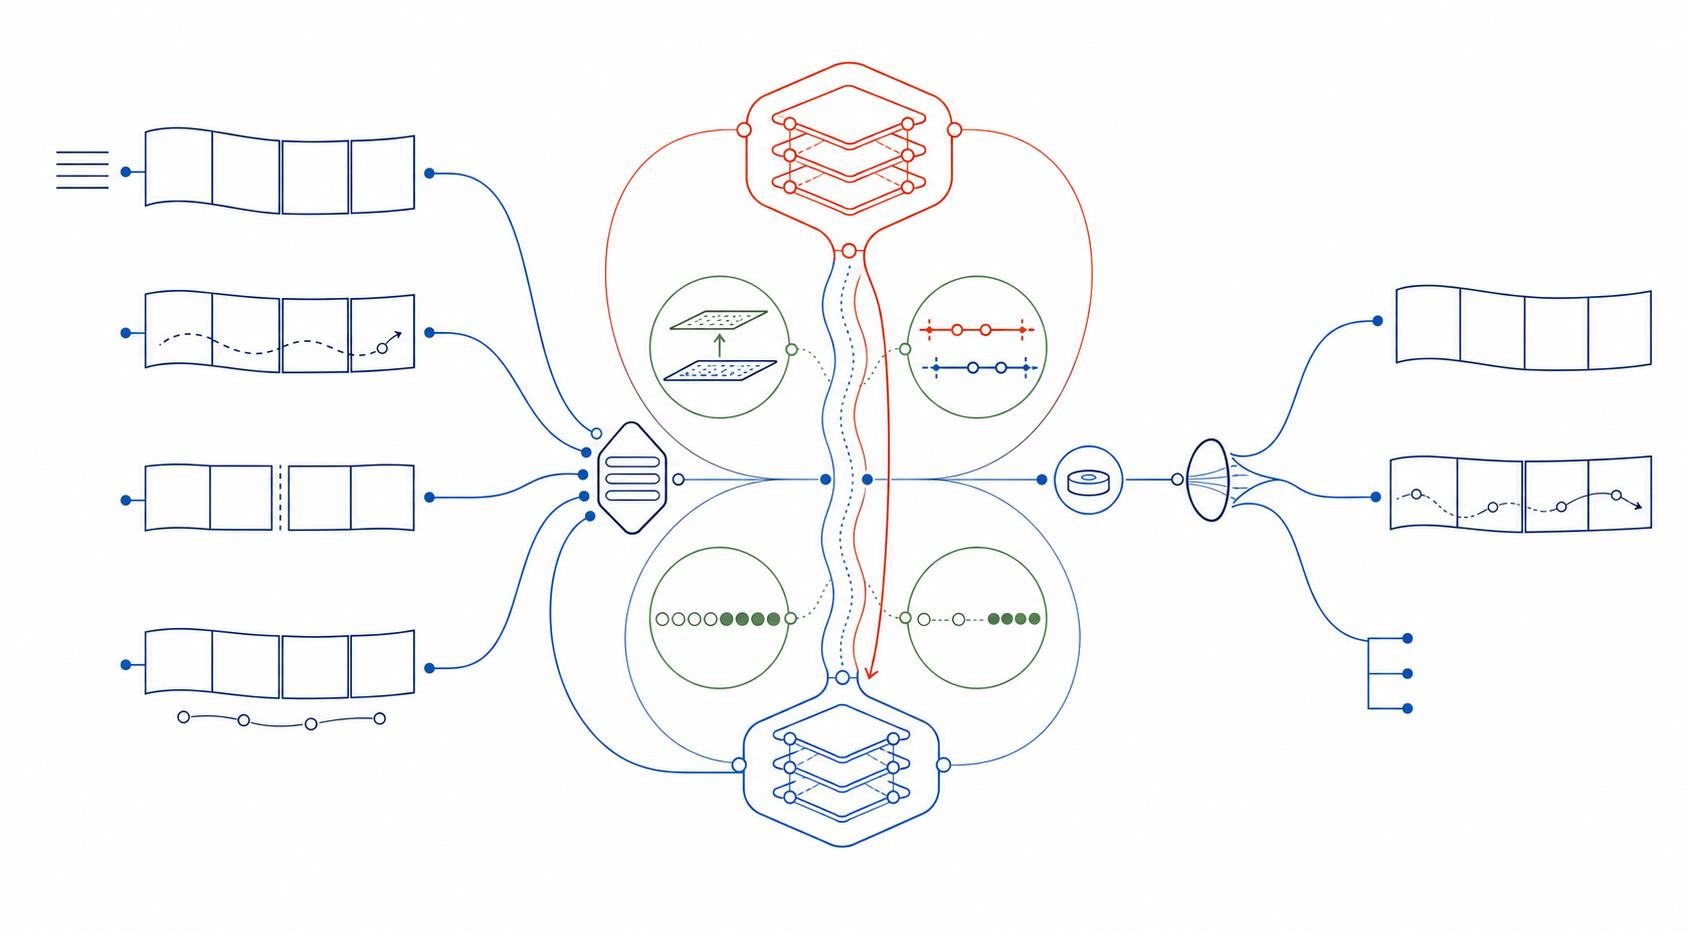
\includegraphics[width=16cm]{overview_assets/bowtie_base.png}
  };
  \begin{scope}[x={(image.south east)},y={(image.north west)}]
    % Preserve the approved bow-tie core and replace only the generic side strips.
    \fill[white] (0.020,0.748) rectangle (0.249,0.872);
    \fill[white] (0.020,0.566) rectangle (0.249,0.696);
    \fill[white] (0.020,0.392) rectangle (0.249,0.523);
    \fill[white] (0.020,0.158) rectangle (0.249,0.337);
    \fill[white] (0.823,0.575) rectangle (0.998,0.795);
    \fill[white] (0.823,0.360) rectangle (0.998,0.588);

    % Task-specific input motifs.
    \node[inner sep=0] at (0.137,0.810) {
      
\includegraphics[width=3.50cm]{overview_assets/text_to_video.png}
    };
    \node[inner sep=0] at (0.137,0.630) {
      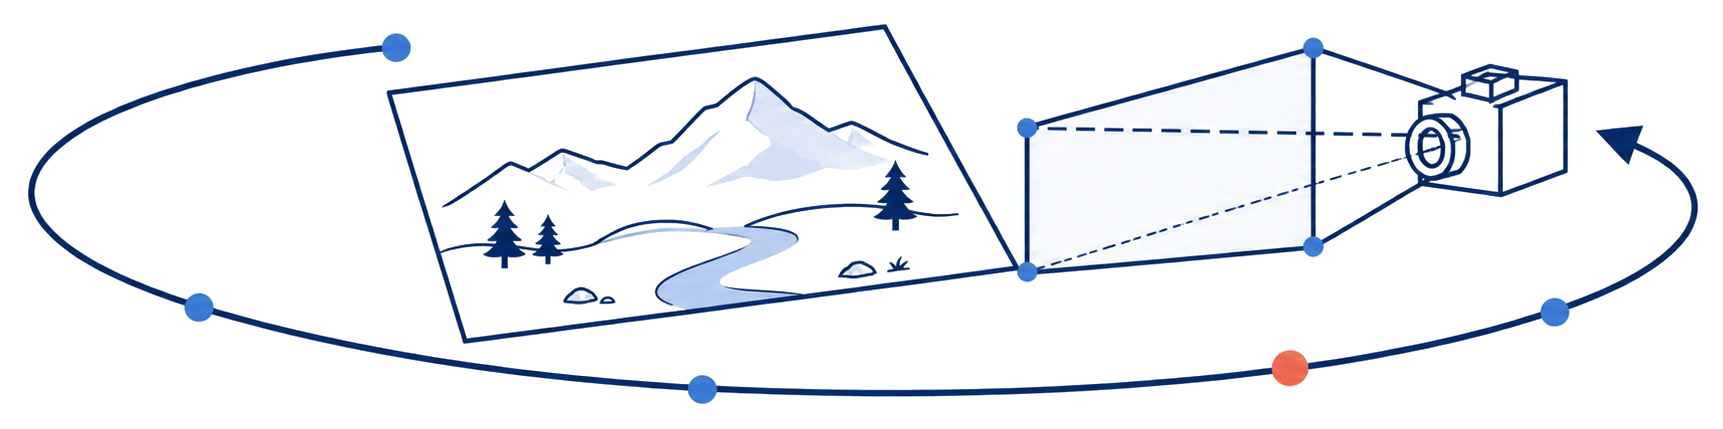
\includegraphics[width=3.48cm]{overview_assets/image_camera_control.png}
    };
    \node[inner sep=0] at (0.137,0.458) {
      
\includegraphics[width=3.50cm]{overview_assets/streaming_long_video.png}
    };
    \node[inner sep=0] at (0.137,0.247) {
      
\includegraphics[width=3.46cm]{overview_assets/action_conditioned_rollout.png}
    };

    % Output-specific motifs.
    \node[inner sep=0] at (0.909,0.700) {
      
\includegraphics[width=2.58cm]{overview_assets/generated_video.png}
    };
    \node[inner sep=0] at (0.909,0.490) {
      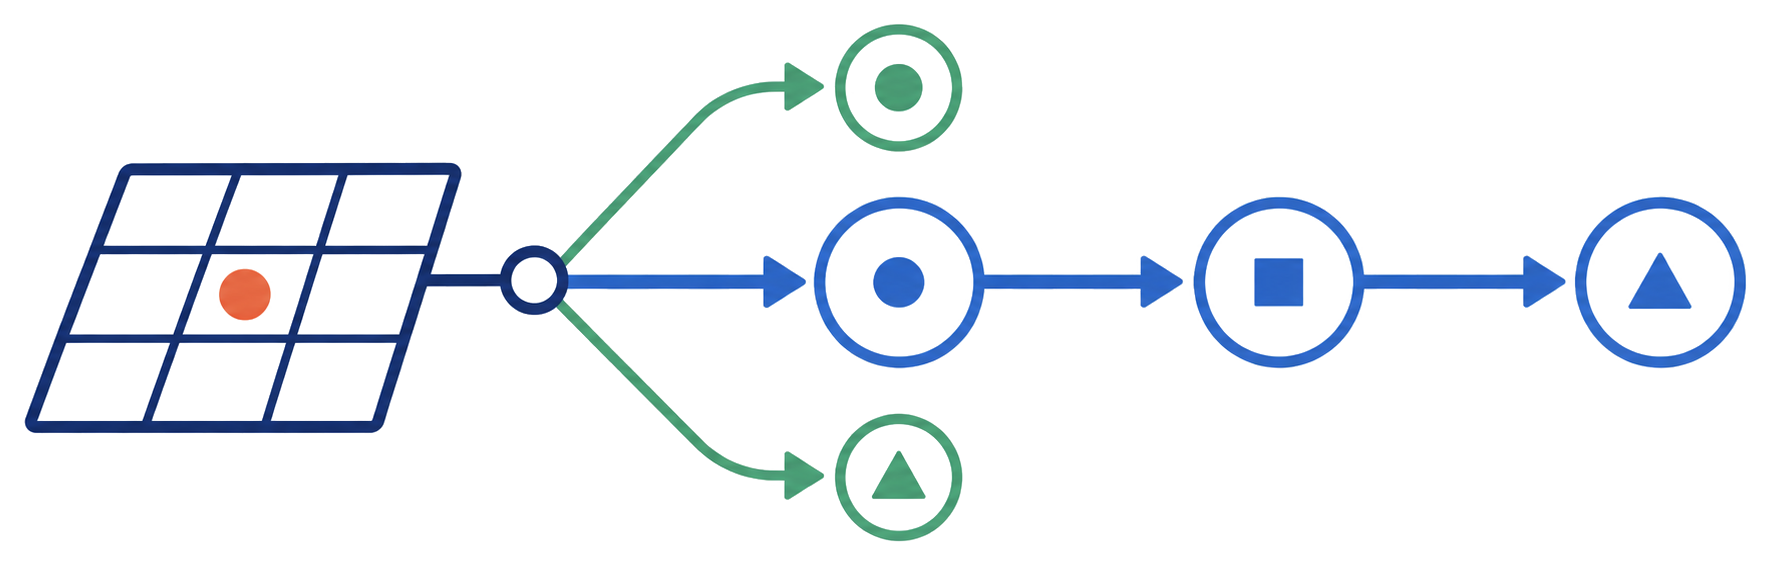
\includegraphics[width=2.78cm]{overview_assets/world_model_rollout.png}
    };

    % Four standardized task/data streams.
    \node[labelbox,text=ink,font=\fontsize{5.4}{6.2}\selectfont\bfseries] at (0.145,0.922)
      {Text-to-Video};
    \node[labelbox,text=ink,font=\fontsize{5.4}{6.2}\selectfont\bfseries] at (0.145,0.739)
      {Image / Camera Control};
    \node[labelbox,text=ink,font=\fontsize{5.4}{6.2}\selectfont\bfseries] at (0.145,0.562)
      {Streaming Long Video};
    \node[labelbox,text=ink,font=\fontsize{5.4}{6.2}\selectfont\bfseries] at (0.145,0.357)
      {Action-Conditioned Rollout};

    % Shared metadata and teacher/student pair.
    \node[labelbox,text=student,font=\fontsize{5.6}{6.4}\selectfont\bfseries] at (0.365,0.585)
      {Canonical Model Catalog\\[-1pt]\fontsize{4.5}{5.2}\selectfont aliases $\cdot$ runner $\cdot$ pairing};
    \node[labelbox,text=teacher,font=\fontsize{6.6}{7.4}\selectfont\bfseries] at (0.500,0.955)
      {Teacher $v_{\theta_t}$};
    \node[labelbox,text=student,font=\fontsize{6.6}{7.4}\selectfont\bfseries] at (0.500,0.070)
      {Student $v_{\theta_s}$};

    % Four code-aligned runtime policies.
    \node[labelbox,text=runtime,font=\fontsize{5.4}{6.2}\selectfont\bfseries] at (0.425,0.735)
      {Hot / Cold Cache\\[-1pt]\fontsize{4.4}{5.2}\selectfont freshness $g_{\Delta}$};
    \node[labelbox,text=runtime,font=\fontsize{5.4}{6.2}\selectfont\bfseries] at (0.580,0.735)
      {Async CUDA Streams\\[-1pt]\fontsize{4.4}{5.2}\selectfont overlap $\alpha$};
    \node[labelbox,text=runtime,font=\fontsize{5.4}{6.2}\selectfont\bfseries] at (0.425,0.245)
      {Target-Only Mask\\[-1pt]\fontsize{4.4}{5.2}\selectfont $M_{\pi}=[0_{\mathrm{ctx}},1_{\mathrm{tgt}}]$};
    \node[labelbox,text=runtime,font=\fontsize{5.4}{6.2}\selectfont\bfseries] at (0.580,0.245)
      {Hybrid-Sparse Memory\\[-1pt]\fontsize{4.4}{5.2}\selectfont budget $B$, recent ratio $\rho$};

    % Supervision and deployment path.
    \node[plainlabel,text=teacher,font=\fontsize{4.6}{5.4}\selectfont\bfseries,rotate=90] at (0.520,0.505)
      {$\operatorname{sg}(v_{\theta_t})$ supervision};
    \node[labelbox,text=student,font=\fontsize{5.2}{6.0}\selectfont\bfseries] at (0.657,0.430)
      {Distilled Student\\Checkpoint};
    \node[labelbox,text=student,font=\fontsize{5.2}{6.0}\selectfont\bfseries] at (0.735,0.585)
      {Shared Runner\\+ Scheduler};
    \node[labelbox,text=student,font=\fontsize{5.2}{6.0}\selectfont\bfseries] at (0.909,0.810)
      {Generated Video};
    \node[labelbox,text=student,font=\fontsize{5.2}{6.0}\selectfont\bfseries] at (0.909,0.386)
      {World-Model Rollout};
    \node[labelbox,text=ink,font=\fontsize{5.0}{5.8}\selectfont\bfseries] at (0.865,0.215)
      {CLI $\cdot$ REST $\cdot$ UI};

    % Compact objective family: the shared interface does not imply one universal loss.
    \node[objectivebox,text=ink,font=\fontsize{4.05}{4.95}\selectfont,text width=3.90cm] at (0.775,0.900) {
      {\bfseries Trainer-Specific Objectives}\\[-1pt]
      $\displaystyle
        \mathcal{L}_{\mathrm{trainer}}
        =\mathcal{L}_{\mathrm{task}}(M_{\pi})
        +\lambda_{\mathrm{aux}}\mathcal{L}_{\mathrm{aux}}
      $\\[-1pt]
      \fontsize{3.55}{4.25}\selectfont
      task: reg $\cdot$ prog $\cdot$ cons
      $\;\vert\;$ aux: adv $\cdot$ DMD
    };

    % Method choices are parallel registry entries, not a serial pipeline.
    \node[labelbox,text=ink,font=\fontsize{4.8}{5.8}\selectfont\bfseries] at (0.500,0.018) {
      Trainer Registry:
      Step $\cdot$ Progressive $\cdot$ Consistency $\cdot$ Stream $\cdot$
      Context Forcing $\cdot$ ADD/LADD $\cdot$ DMD/DMD2
    };
  \end{scope}
\end{tikzpicture}
\end{document}
